%! Author = marti
%! Date = 4/28/2021

% Preamble
\documentclass[11pt]{article}

% Packages
\usepackage{amsmath}
\usepackage{graphicx}
\graphicspath{ {./images/}}

% Document
\begin{document}
    \bibliography{main}
    \bibliographystyle{plain}


    \section{Data}
    We have exported the data from the ExCape database.
    The web interface provides both a web interface for data exploration and export, and an API to query the database.
    The documentation of the former is unfortunately not available, and the latter fails on export of larger datasets.
    As such we have exported the data using our own tool which is available at https://github.com/B1RO/ExcapeDBDownloader.
    The graph bellow shows the gene targets with the largest facet counts - the number of small molecules measured for a given gene target.
    \begin{figure}[h!]
        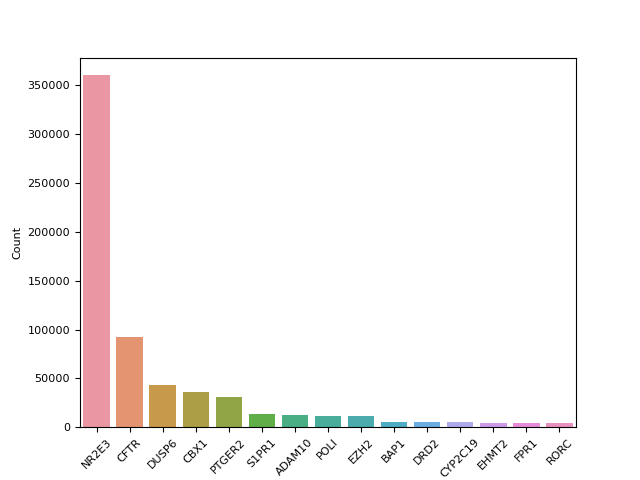
\includegraphics{target_counts}
        \label{fig:target_counts}
    \end{figure}

    In practice when we export data from the database a larger number of items seems to be returned than the facet count would indicate.
    However the facet counts still serve as a good indicator of the relative number of data per gene target.
    For our exploratory data analysis we have chosen the last 5 genes in the graph (RORC, FPR1, EHMT2, CYP2C19, DRD2).
    In total these 5 genes consist of 396762 data samples, where each sample is a json object with the following fields:
    \begin{itemize}
        \item \text{Original\_Entry\_ID}
        \item \text{Entrez\_ID}
        \item \text{Activity\_Flag} - either 'N' - inactive or 'A' - active
        \item DB - the ExCAPE database consists of multiple source databases, this field signifies which database the data originate from
        \item \text{Original\_Assay\_ID}
        \item \text{Tax\_ID} - identifies the species that the small molecule was tested against by it's unique taxonomy id, searchable on ncbi.nlm.nih.gov/taxonomy.
        \item \text{Gene\_Symbol} - unique symbol of the gene
        \item \text{Ortholog\_group} - orthological group of the gene
        \item \text{SMILES} - description of the chemical species using short ASCII strings.
        \item \text{Ambit\_InchiKey} - hashed international chemical identifier
    \end{itemize}

    To obtain predictor variables for machine learning we use the RDKit and mordred library.
    All variables are extracted from the SMILES field. The SMILES field is first transformed into RDKit's molecular representation of those smiles.
    Some SMILE strings are deemed chemically unreasonable
    by RDkit, and we disregard those in further analysis.
    The molecular representations are then converted into ~1800 molecular descriptors using the
    mordred library.

    Further analysis shows that many descriptors are stored as strings and not numerical values.
    This is caused by missing values. Some columns contain no, or a very small amount of
    numerical data points. Given the number of training features available, we simply drop all columns that have more than 2.5% values missing. Other columns are
    filled by a forward fill.
    The data are then exported into the .svmlight format.


\end{document}
